\subsection{Design patterns}\label{sec:design_pattern_individual_proxyapps}
\subsubsection{Template Method}\label{sec:template}

The Template Method involves the implementation of an algorithm as a carcass with interchangeable components, deferring some of the components to subclasses; thus steps in an algorithm can be redefined while retaining the overall algorithm structure.  
Code outside the class hierarchy sees a common interface: the public function in the base class, the implementation of which contains the invariant parts of the algorithm, thereby avoiding code duplication.  
A selection of protected virtual component functions may be called by other classes in the inheritance hierarchy. 

%any other wisdom in Go4:
This design pattern is such a fundamental technique for code reuse that it is likely to be applicable to an extremely wide range of object-oriented codes.  
In {\it Nektar++} it is used, to take just one example, to enable the quadrature of functions over the regions defined by differently-shaped finite elements.
In BOUT++, this is used to perform the same operation on arrays of different type, so that there is no need to repeat the definition of, say, elementwise addition for \texttt{int}, \texttt{float} and \texttt{double}.

A UML representation of this pattern can be seen in Fig.\ref{fig:templatemethoduml} (note that all UML - and other - diagrams used in this report were constructed using the free graphing software {\it yEd} \cite{yedwebsite}).

\begin{figure}
\centerline{\rotatebox{0}{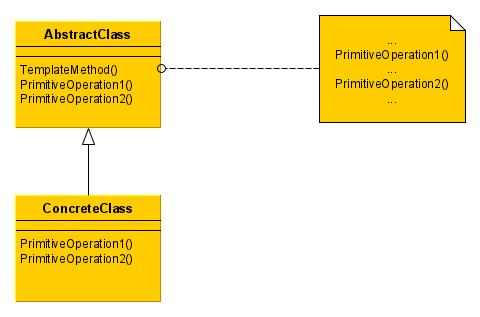
\includegraphics[width=12cm]{../png/templatemethod.jpg}}}
\caption{\label{fig:templatemethoduml}
UML diagram for the Template Method pattern.}
\end{figure}

\subsubsection{Abstract Factory}\label{sec:abstract_factory}

Factories are used to create instances of classes using class-specific creator functions; the objects created are of some derived type but are returned as a base-class pointer.  
This has obvious benefits, for example that the users of factory-created objects need only focus on those objects' interfaces and not the specifics of individual implementations; also, header-file dependencies are reduced, improving compile times.

Another very useful thing this enables is the disabling of certain implementations (e.g. relating to third-party libraries) during the build process; one simply avoids compiling unwanted implementations, rather than needing preprocessing flags to be insinuated throughout the code.

Abstract Factories are used in BOUT++ to allow different computational meshes.
This allows the details and implementation to vary quite dramatically (compare,
for example, a uniform grid and a completely unstructured mesh), while still
exposing fundamentally the same \texttt{mesh} object to the rest of the code.

%any other wisdom in Go4:

\begin{figure}
\centerline{\rotatebox{0}{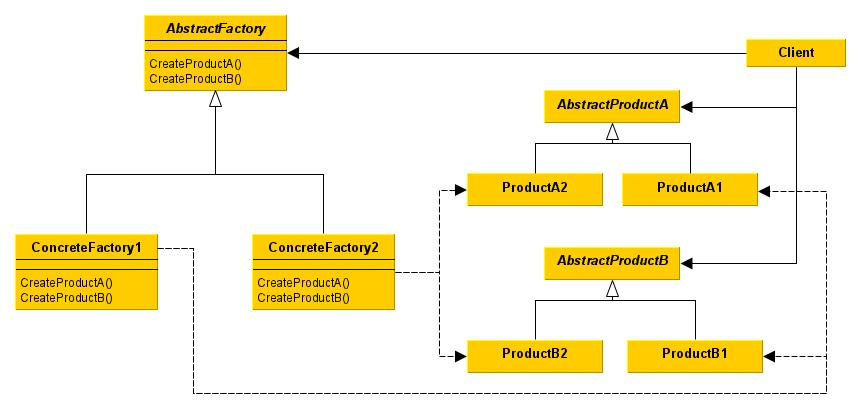
\includegraphics[width=12cm]{../png/abstractfactory.jpg}}}
\caption{\label{fig:abstractfactoryuml}
UML diagram for the Abstract Factory pattern.}
\end{figure}

\subsubsection{Strategy}\label{sec:strategy}

The Strategy pattern uses delegation to vary an entire algorithm (compare the Template Method described above, which varies only part of the algorithm, in a particular way).

One salient example of this is an interchangeable matrix-free Laplacian kernel intended to supersede the existing (non-matrix-free) x86 implementation in {\it Nektar++}: upcoming work will focus on implementing vectorized x86, GPU, and ARM versions of the compute kernel.  
Here, the Strategy pattern provides an alternative to a layered architecture in enabling performance portability.

This pattern is also used in BOUT++ to implement different elliptic solvers.
Thus a PETSc or Hypre solver will be implemented in the proxyapp as a new
``concrete strategy'' in BOUT++'s \texttt{Laplacian} class; essentially an
inherited class that provides an overload to the function
\texttt{Laplacian->solve} which inverts the elliptic operator using the library
solver.

%Go4:

\begin{figure}
\centerline{\rotatebox{0}{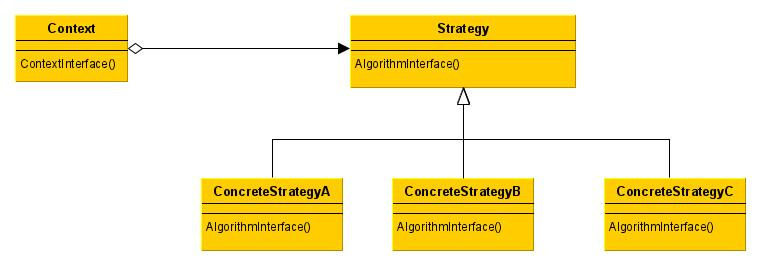
\includegraphics[width=12cm]{../png/strategy.jpg}}}
\caption{\label{fig:strategyuml}
UML diagram for the Strategy pattern.}
\end{figure}

\subsubsection{Flyweight}

The Flyweight pattern is a means to allow object fine-graining whilst avoiding prohibitively large storage costs.  
A reference to a shared object (or the shared parts of an object) are used instead of the object; in this way, the unnecessary duplication of potentially large data objects is avoided.  
The shared quantity is referred to as the Flyweight (with mild irony, as these objects may actually be very large).

A specific example in certain types of finite-element code is the storage of the various finite-element matrices needed by each element (and of the latter there may be millions); these matrices involve a table of integrals of basis function bilinears indexed by the row and column of the matrix.  
The need to store a copy of the matrix for each element can be avoided, in some cases, by storing a global reference matrix and adapting this to each specific element by means of an element-specific mapping (typically using a handful of parameters specific to the geometry of the individual element).

This pattern is ubiquitous in systems containing large numbers of facsimile or closely-related objects.  
Note there are also considerations relating to how the objects might be created and managed taking into account the need to avoid duplication and these are illustrated in the UML diagram in Fig.\ref{fig:flyweightuml}.

\begin{figure}
\centerline{\rotatebox{0}{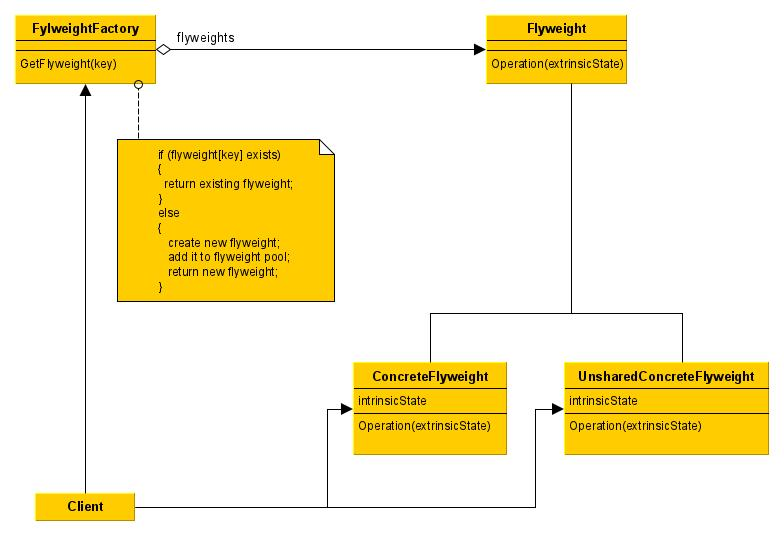
\includegraphics[width=12cm]{../png/flyweight.jpg}}}
\caption{\label{fig:flyweightuml}
UML diagram for the Flyweight pattern.}
\end{figure}

\subsubsection{Pipeline}

The {\it NekMesh} framework is implemented as a set of modules which operate sequentially on the mesh data in an example of the pipeline architectural pattern.  See \ref{fig:pipeline}.

\begin{figure}
\centerline{\rotatebox{0}{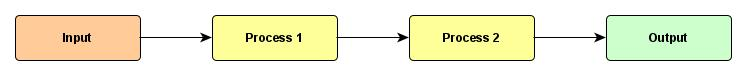
\includegraphics[width=12cm]{../png/pipeline.jpg}}}
\caption{\label{fig:pipeline}
Illustrative pipeline of the {\it NekMesh} process.  Reproduced from Figure 4.2 of the User Guide obtainable from \cite{nektarwebsite}.}
\end{figure}

\subsubsection{Modular design}\label{sec:modular}

The modular design pattern organizes source code into components called
modules, where each module is a collection of code necessary to achieve a
particular task.
Variables may be local to a function within a module,
or they may be module-level, that is, available for reading and writing to all
functions in that module.
Further, when given the \texttt{public} attribute (in Fortran), module-level
variables may be edited by \emph{all} modules.
Different modules may interact via public variables, however it is better practice for
all interaction to take place using function calls, even if these only trivially
return the valuable of one variable from within another module. 

Modules must also be self initializing and finalizing, providing routines that
are equivalent to constructors and destructors in object-oriented programming.
It is the existence of constructors and destructors that distinguishes a module
from a namespace.

GS2 makes use of modules, with different physical effects (e.g. collisions,
$E\times B$ advection) and infrastructure (e.g. meshing, I/O), each existing
within its own module.



\subsubsection{Lazy initialization}\label{sec:lazy_init}

Lazy initialization is the technique of delaying the call to an object's
constructor or a module's initialization function until just before its first
use.
This allows faster speeds and lower memory consumption during code
initialization, though this is a spreading of cost throughout the code's
execution rather than a saving.

It also allows for a passive approach to managing dependencies between objects.
For example, GS2 does not handle the dependences between modules explicitly in
its initialization phase.
Instead, each module's initialization subroutine \texttt{init} begins by
calling the \texttt{init} routine of all the module's dependencies, before
going on to initialize itself.
Repeat initializations are prevented using a module-level \texttt{initialized}
logical variable in each module.
A similar approach is taken to uninitialization.
This approach requires a developer to have some sense of the dependencies
between modules in order to avoid compilation errors due to circular
dependencies.
However, dependencies are often straightforward, and this approach is very
lightweight and easy-to-use compared to an explicit approach to managing module
dependencies.


\subsubsection{Dependency injection}\label{sec:dependency_injection}

Dependency injection is a technique where a function or subroutine receives its
dependencies as input arguments.
The function receiving the dependency is called a client, and the dependency
received is called a service.
In this approach, the client is able to use whatever dependency is passed to it, 
rather than needing to specify or create the dependencies itself.
The advantage of dependency injection is that it allows separation of concerns --
the client uses the service, but some other part of the code creates the service --
increasing readability and code reuse.

Dependency injection also provides a means for older codes like GS2 to
incorporate object-oriented patterns without completely rewriting legacy code.
In GS2, some objects that were previously module-level variables are instead
wrapped into a large \texttt{state} object.
The \texttt{state} is then the input/output of subroutines, allowing the
module-level variables to be incrementally removed.
